\documentclass[10pt]{article}

%\usepackage{hyperref}
\usepackage{alltt}
\usepackage{natbib}
\usepackage{graphicx}
\usepackage{url}
\usepackage{fancyhdr}
\usepackage{trust}
\pagestyle{fancy}

\usepackage{tikz}
\usetikzlibrary{arrows,shadows}
\usepackage[underline=false]{pgf-umlsd}

\lhead{}
\rhead{}
\lfoot{\copyright The University of Kansas, 2012}
\cfoot{\thepage}


\newtheorem{conjecture}{Conjecture}
\newtheorem{obligation}{Obligation}
\newtheorem{definition}{Definition}


\usepackage{ifthen}
\newboolean{submission}  %%set to true for the submission version
\setboolean{submission}{false}
%\setboolean{submission}{true}
\ifthenelse
{\boolean{submission}}
{ \newcommand{\todo}[1]{ } } % hide todo
{ \newcommand{\todo}[1]{ % show todo
   \marginpar{\raggedright\footnotesize{#1}}
               }}

\parskip=\medskipamount
\parindent=0pt

\bibliographystyle{abbrvnat}

\title{ArmoredSoftware Architecture}
\author{Perry Alexander \and Andy Gill \and Prasad Kuklarni \and Leon
  Searl \\
Information and Telecommunication Technology Center \\
The University of Kansas \\
\url{{palexand,andygill,prasadk,lsearl}@ku.edu}}

\begin{document}

\maketitle
\tableofcontents
\listoffigures
\listoftables

\begin{abstract}
  This document describes the evolving ArmoredSoftware architecture.
\end{abstract}

\section{Introduction}

The objective of \textsc{ArmoredSoftware} is to \emph{provide a portable
trusted computing capsule for applications executing in the cloud}.
This capsule, referred to as \emph{armor}, provides three major
functions:

\begin{description}
  \parskip=0pt\itemsep=0pt
\item[Appraisal] -- Request and assess measurement information from
  the operational environment and other armored components.
\item[Measurement] -- Gather run-time measurement information from its
  application
\item[Attestation] -- Assemble and deliver evidence to appraisers in a
  manner that assures measurement integrity
\end{description}

Figure~\ref{fig:architecture} graphically depicts the major
architectural components of a protected application.  The
\emph{application} is the application to be protected by the
infrastructure.  The \emph{measurement} component performs measurement
operations on the running application while the \emph{attestation}
component gathers measurements and delivers them with cryptographic
assurance of integrity and confidentiality.  The \emph{appraisal}
component requests information from the environment and other
components to assess the overall operational environment.
\emph{Access control} governs access to all critical resources in the
protected application to assure secrets are preserved and enforce
information flow restrictions.

\begin{figure}
  \centering
  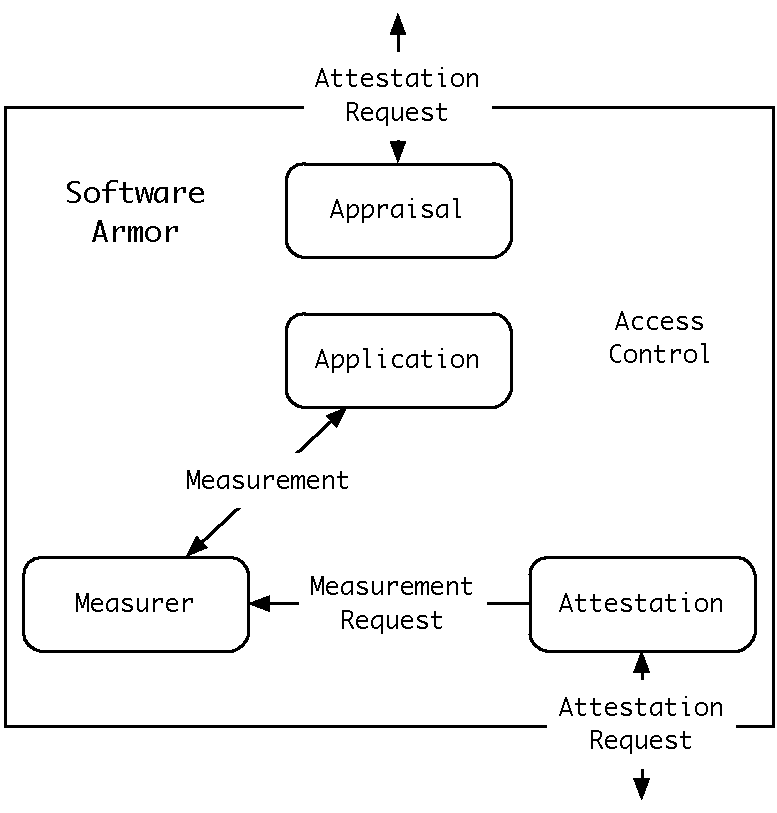
\includegraphics[width=0.5\textwidth]{figures/architecture.pdf}
  \caption{AS Architecture}
  \label{fig:architecture}
\end{figure}

Figure~\ref{fig:system} graphically represents the interaction among
protected components while figure~\ref{fig:sequence} shows the
sequencing of interactions during appraisal.  A component's appraisal
module will request information from a second component's attestation
module.  The attestation model will select an attestation protocol
that instructs the measurer what information to gather and in what
sequence.  The attestation module packages measurement results in a
evidence packet that is return to the appraiser requesting
information.  The appraiser then assesses cryptographic signatures and
encryption to determine the trustworthiness of the measurements, then
assesses measurements to determine the trustworthiness of the
component being appraised.  Note that the same process occurs when
appraising the component's operational environment.

\begin{figure}[hbtp]
  \centering
  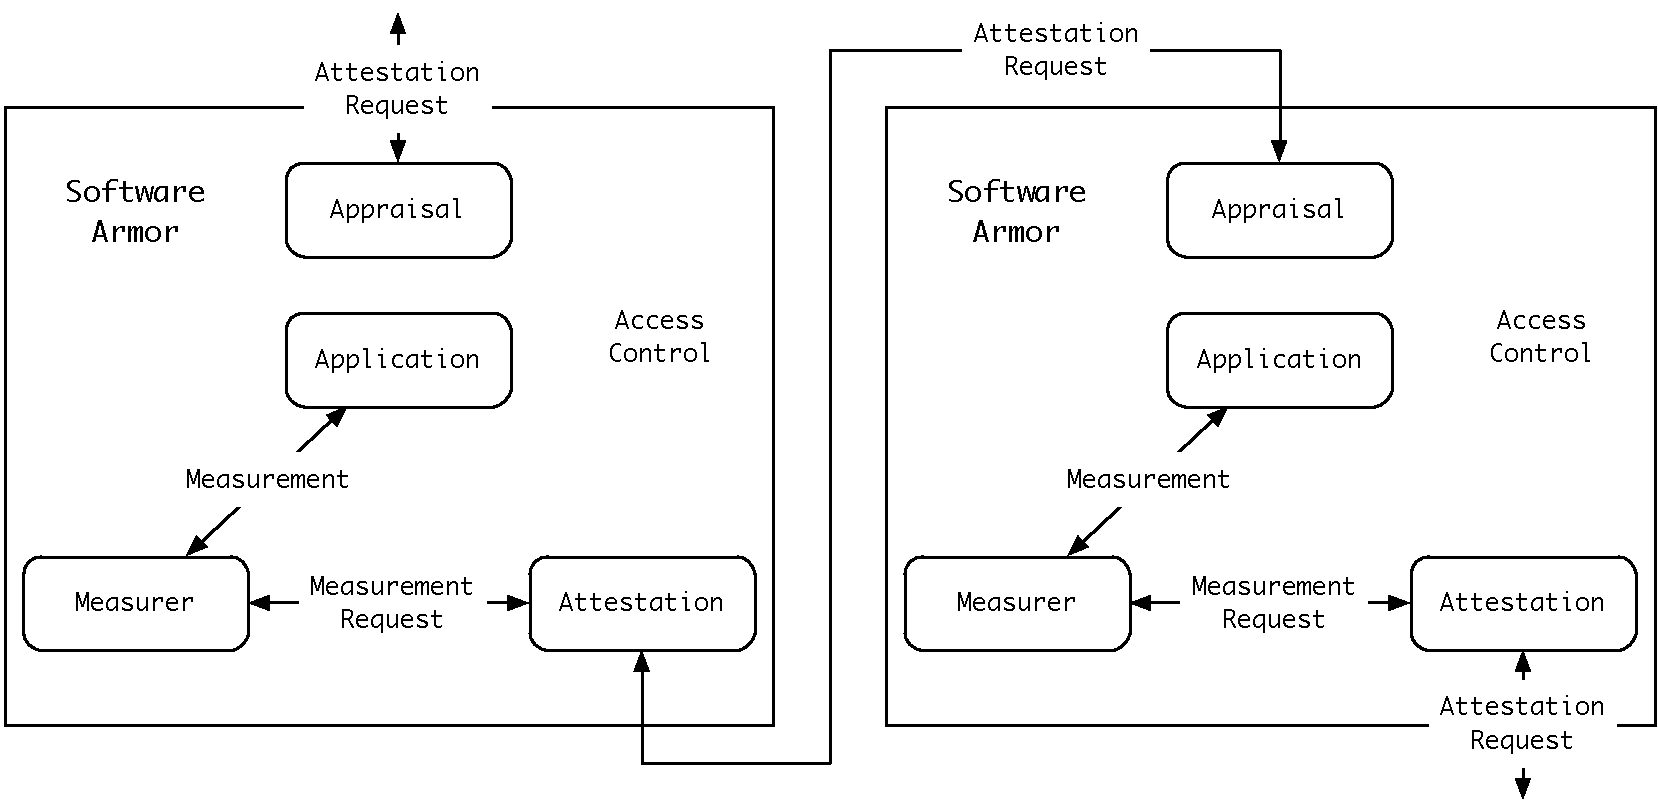
\includegraphics[width=0.5\textwidth]{figures/system.pdf}
  \caption{System Architecture}
  \label{fig:system}
\end{figure}

\begin{figure}
\begin{footnotesize}
  \begin{sequencediagram}
    \newthread[white]{appr}{Appraiser}
    \newinst[2]{attest}{Attestation}
    \newinst[2]{meas}{Measurer}
    \newinst[2]{app}{Application}
    
    \begin{call}{appr}{Attestation Request}{attest}{Attestation}
      \begin{callself}{attest}{Protocol Selection}{Attestation Preparation}
      \begin{call}{attest}{Measurement Requests}{meas}{Measurement Values}
        \begin{call}{meas}{Measurement Calls}{app}{Measurement Values}
        \end{call}
      \end{call}
      \end{callself}
    \end{call}
    \begin{callself}{appr}{Appraisal}{Execute Decision}
    \end{callself}
  \end{sequencediagram}
\end{footnotesize}
\caption{Architecture component interaction}
\label{fig:sequence}
\end{figure}

\section{System Architecture}

\subsection{Measurement}

\subsection{Attestation}

Figure~\ref{fig:attestation-1} graphically shows the processing of an
attestation request by an ArmoredSoftware attestation component.  The
attestation request specifies information requested by an appraiser.
Upon receipt, the \emph{Attestation Protocol Selector} or \emph{AP
  Selector} identifies one or more \emph{Attestation Protocols} that
could satisfy the appraisers request.  The protocol is passed to the
\emph{AP Instantiation} process that selects specific mechanisms for
achieving individual requests in the AP.  The resulting protocol
instance is passed to \emph{AP Execution} where it is executed by: (i)
making requests to the component's vTPM; making requests to another
components attestation service; or (iii) invoking the measurer on the
component's associated application.

\begin{figure}[hbtp]
  \centering
  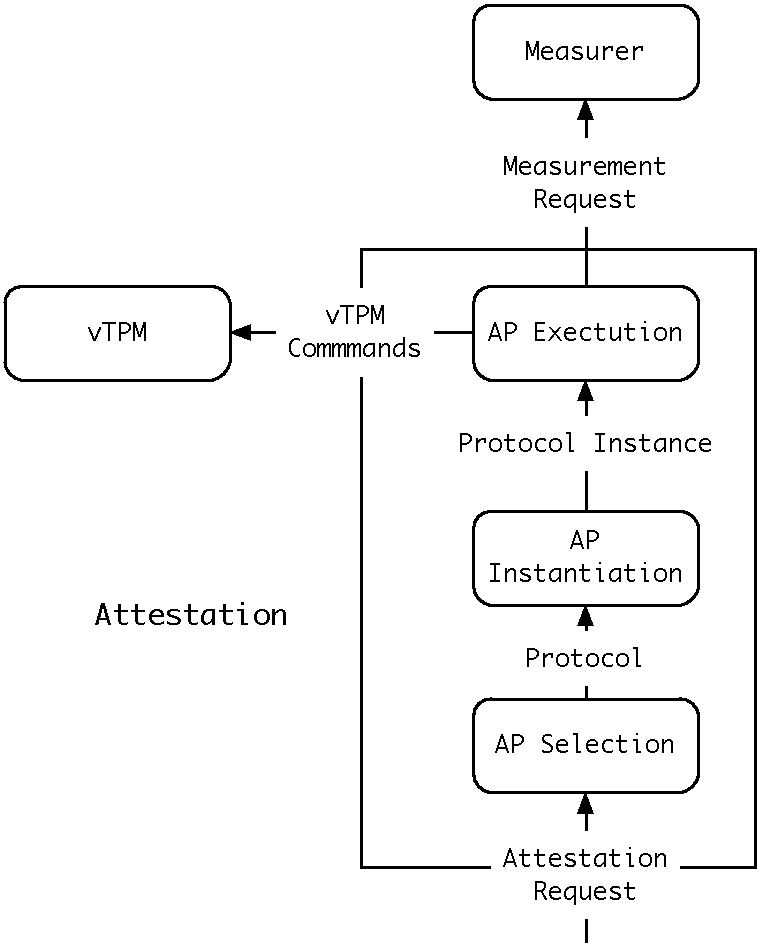
\includegraphics[width=0.50\textwidth]{figures/attestation-1.pdf}
  \caption{Attestation request processing}
  \label{fig:attestation-1}
\end{figure}

The results of request to the vTPM, another attestation component, and
the local measurer are returned as vTPM quotes, evidence packages, and
measurements respectively.  The AP Execution component monitors
execution and collects various results for processing by the AP
Instantiation component.  AP Instantiation assembles individual
measurement, vTPM and appraisal results into a package representing
information requested in the attestation request.  The AP Selection
component uses cryptographic techniques to provide assurances to the
appraiser requesting information that evidence can be trusted.
Finally, the evidence package is returned to the requesting appraiser
where it is evaluated.

\begin{figure}[hbtp]
  \centering
  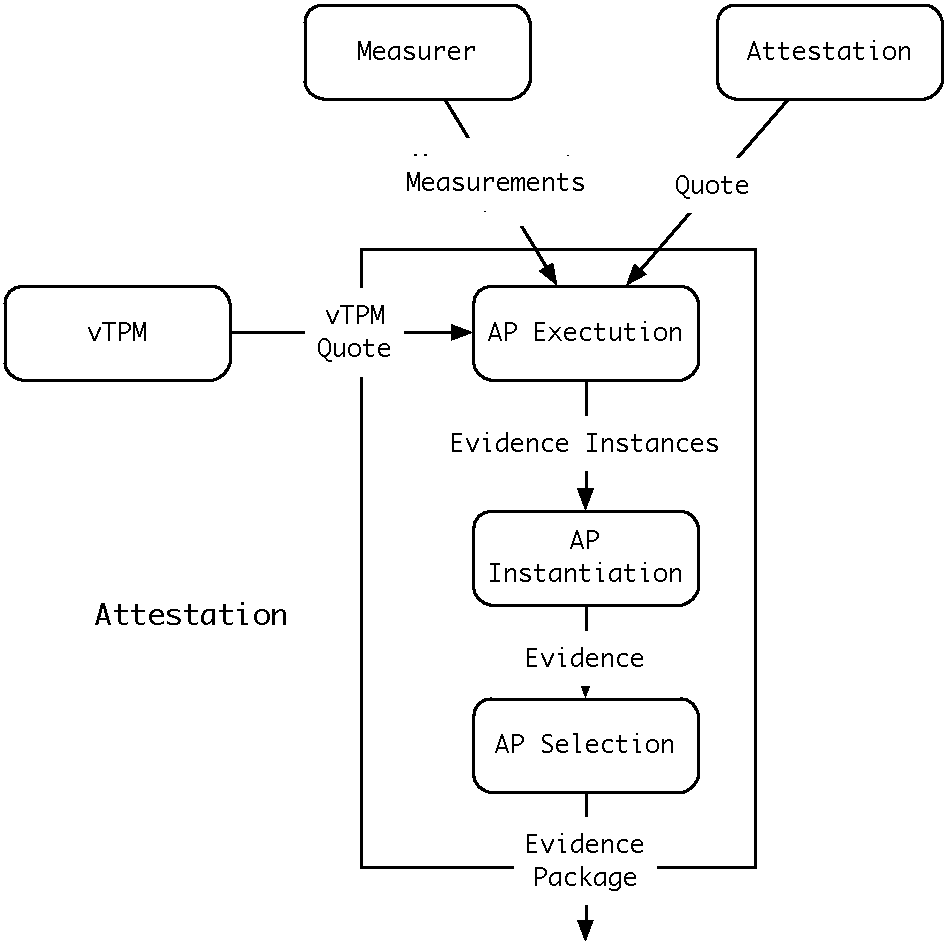
\includegraphics[width=0.50\textwidth]{figures/attestation-2.pdf}
  \caption{Attestation evidence processing}
  \label{fig:attestation-2}
\end{figure}

\subsubsection{TPM and vTPM}

\subsection{Appraisal}

\subsubsection{Migration}

\subsection{Access Control}

\section{Component Interaction}

\appendix

%%\input{glossary}

%%\nocite{}

\bibliography{sldg}

\end{document}
